% ---------------------------------------------------------------------------
% Quelle der Abbildung:
%   Skript:  thesis/figures/scripts/hologramm_simulation.py (eigene Fresnel-Simulation,
%            N = 512, Padding 2, kein Trainingslauf, kein HoloForge-Datensatz)
%   Aufruf:  /tmp/holo311/bin/python thesis/figures/scripts/hologramm_simulation.py
%   Basis:   Commit 1abccf9 (Branch cursor/thesis-grundlagen-6175), 2026-10-01
%   Dateien: radialprofil_spektrum.pdf (dasselbe Skript erzeugt
%            figures/grundlagen/hologramm_spektrum.pdf)
% Einbinden im Kapitel: % ---------------------------------------------------------------------------
% Quelle der Abbildung:
%   Skript:  thesis/figures/scripts/hologramm_simulation.py (eigene Fresnel-Simulation,
%            N = 512, Padding 2, kein Trainingslauf, kein HoloForge-Datensatz)
%   Aufruf:  /tmp/holo311/bin/python thesis/figures/scripts/hologramm_simulation.py
%   Basis:   Commit 1abccf9 (Branch cursor/thesis-grundlagen-6175), 2026-10-01
%   Dateien: radialprofil_spektrum.pdf (dasselbe Skript erzeugt
%            figures/grundlagen/hologramm_spektrum.pdf)
% Einbinden im Kapitel: % ---------------------------------------------------------------------------
% Quelle der Abbildung:
%   Skript:  thesis/figures/scripts/hologramm_simulation.py (eigene Fresnel-Simulation,
%            N = 512, Padding 2, kein Trainingslauf, kein HoloForge-Datensatz)
%   Aufruf:  /tmp/holo311/bin/python thesis/figures/scripts/hologramm_simulation.py
%   Basis:   Commit 1abccf9 (Branch cursor/thesis-grundlagen-6175), 2026-10-01
%   Dateien: radialprofil_spektrum.pdf (dasselbe Skript erzeugt
%            figures/grundlagen/hologramm_spektrum.pdf)
% Einbinden im Kapitel: % ---------------------------------------------------------------------------
% Quelle der Abbildung:
%   Skript:  thesis/figures/scripts/hologramm_simulation.py (eigene Fresnel-Simulation,
%            N = 512, Padding 2, kein Trainingslauf, kein HoloForge-Datensatz)
%   Aufruf:  /tmp/holo311/bin/python thesis/figures/scripts/hologramm_simulation.py
%   Basis:   Commit 1abccf9 (Branch cursor/thesis-grundlagen-6175), 2026-10-01
%   Dateien: radialprofil_spektrum.pdf (dasselbe Skript erzeugt
%            figures/grundlagen/hologramm_spektrum.pdf)
% Einbinden im Kapitel: \input{figures/stand_der_technik/radialprofil_spektrum}
% ---------------------------------------------------------------------------
\begin{figure}[tb]
  \centering
  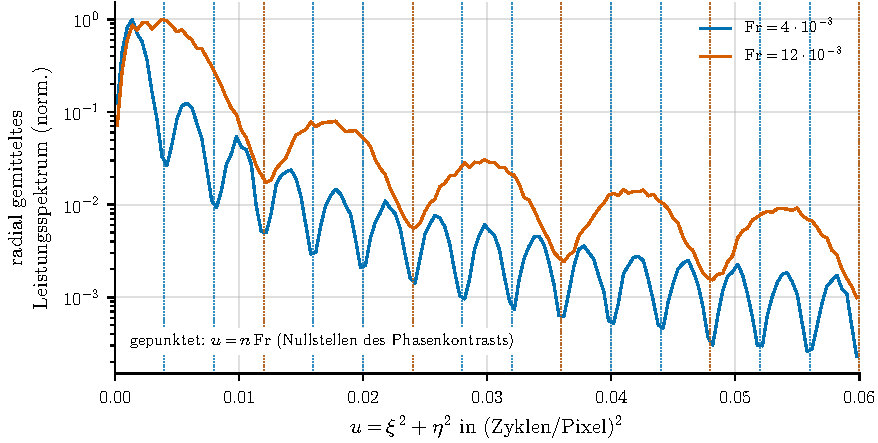
\includegraphics[width=\textwidth]{figures/stand_der_technik/radialprofil_spektrum}
  \caption[Radial gemitteltes Leistungsspektrum simulierter Hologramme über $\xi^2+\eta^2$]{%
    Radial gemitteltes Leistungsspektrum der simulierten Hologramme des schwachen
    Phasenobjekts aus \cref{fig:grundlagen:hologramm}\,(b,\,e), aufgetragen über
    $u = \xi^2+\eta^2$. In dieser Koordinate liegen die Minima
    äquidistant bei $u = n\,\Fr$ (gepunktete Linien), analog zu den Thon-Ringen,
    aus denen \textsc{CTFFIND4} den Defokus elektronenmikroskopischer Aufnahmen
    schätzt \cite{rohou2015ctffind4}. Die Periode des Musters ist unmittelbar die
    Fresnel-Zahl; das Objektspektrum bestimmt nur die Einhüllende.}
  \label{fig:stand:radialprofil}
\end{figure}

% ---------------------------------------------------------------------------
\begin{figure}[tb]
  \centering
  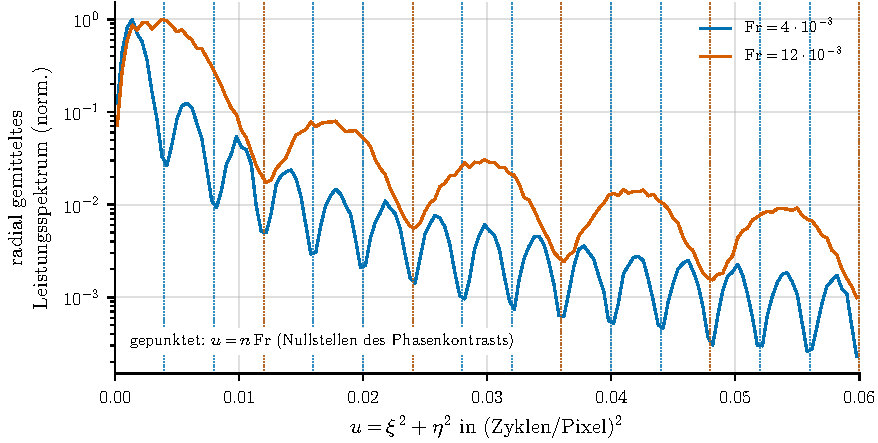
\includegraphics[width=\textwidth]{figures/stand_der_technik/radialprofil_spektrum}
  \caption[Radial gemitteltes Leistungsspektrum simulierter Hologramme über $\xi^2+\eta^2$]{%
    Radial gemitteltes Leistungsspektrum der simulierten Hologramme des schwachen
    Phasenobjekts aus \cref{fig:grundlagen:hologramm}\,(b,\,e), aufgetragen über
    $u = \xi^2+\eta^2$. In dieser Koordinate liegen die Minima
    äquidistant bei $u = n\,\Fr$ (gepunktete Linien), analog zu den Thon-Ringen,
    aus denen \textsc{CTFFIND4} den Defokus elektronenmikroskopischer Aufnahmen
    schätzt \cite{rohou2015ctffind4}. Die Periode des Musters ist unmittelbar die
    Fresnel-Zahl; das Objektspektrum bestimmt nur die Einhüllende.}
  \label{fig:stand:radialprofil}
\end{figure}

% ---------------------------------------------------------------------------
\begin{figure}[tb]
  \centering
  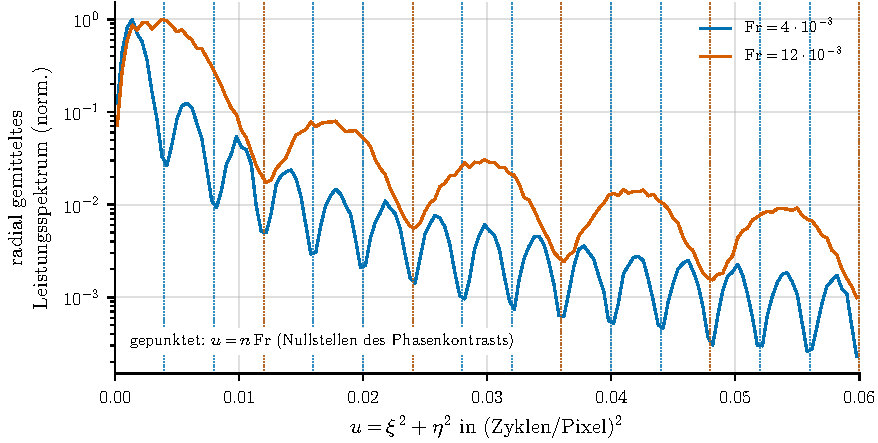
\includegraphics[width=\textwidth]{figures/stand_der_technik/radialprofil_spektrum}
  \caption[Radial gemitteltes Leistungsspektrum simulierter Hologramme über $\xi^2+\eta^2$]{%
    Radial gemitteltes Leistungsspektrum der simulierten Hologramme des schwachen
    Phasenobjekts aus \cref{fig:grundlagen:hologramm}\,(b,\,e), aufgetragen über
    $u = \xi^2+\eta^2$. In dieser Koordinate liegen die Minima
    äquidistant bei $u = n\,\Fr$ (gepunktete Linien), analog zu den Thon-Ringen,
    aus denen \textsc{CTFFIND4} den Defokus elektronenmikroskopischer Aufnahmen
    schätzt \cite{rohou2015ctffind4}. Die Periode des Musters ist unmittelbar die
    Fresnel-Zahl; das Objektspektrum bestimmt nur die Einhüllende.}
  \label{fig:stand:radialprofil}
\end{figure}

% ---------------------------------------------------------------------------
\begin{figure}[tb]
  \centering
  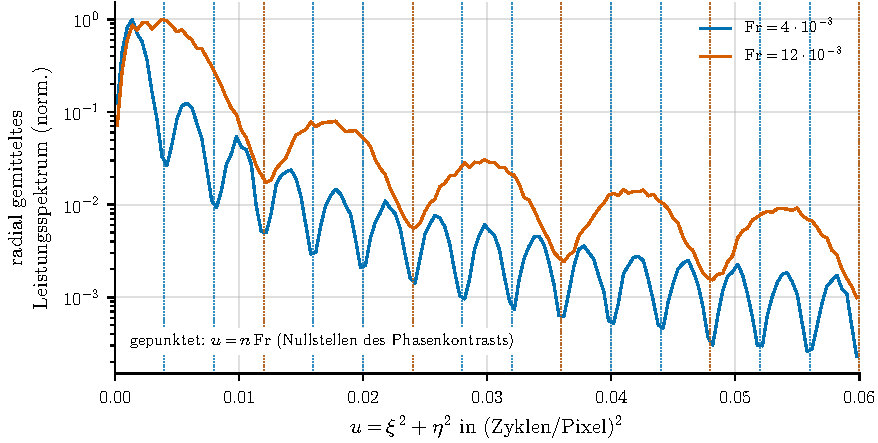
\includegraphics[width=\textwidth]{figures/stand_der_technik/radialprofil_spektrum}
  \caption[Radial gemitteltes Leistungsspektrum simulierter Hologramme über $\xi^2+\eta^2$]{%
    Radial gemitteltes Leistungsspektrum der simulierten Hologramme des schwachen
    Phasenobjekts aus \cref{fig:grundlagen:hologramm}\,(b,\,e), aufgetragen über
    $u = \xi^2+\eta^2$. In dieser Koordinate liegen die Minima
    äquidistant bei $u = n\,\Fr$ (gepunktete Linien), analog zu den Thon-Ringen,
    aus denen \textsc{CTFFIND4} den Defokus elektronenmikroskopischer Aufnahmen
    schätzt \cite{rohou2015ctffind4}. Die Periode des Musters ist unmittelbar die
    Fresnel-Zahl; das Objektspektrum bestimmt nur die Einhüllende.}
  \label{fig:stand:radialprofil}
\end{figure}
